\documentclass{beamer}
\usepackage{epsfig}
\title{Pipelines:  a fundamental building block for efficient hardware}
\author{Madhav P. Desai\\Department of Electrical Engineering\\IIT-Bombay, Mumbai India}
\date{March 8, 2018}
\begin{document}
\maketitle



\frame[containsverbatim]{\frametitle{An example}
\begin{itemize}
\item We want to compute $result(k) = a(k)*(a(k) + 1.0)$ for a sequence of 
numbers. 
\item The system should accept a sequence of numbers $\{a(k))\}$
and produce the sequence $\{ result(k) \}$.
\end{itemize}
}


\frame[containsverbatim]{\frametitle{The program}
\begin{verbatim}
void Daemon()
{
  while(1)
  {
    float a = read_float32("a_pipe");
    float ap1 = (a + 1.0);
    float result = a*ap1;
    write_float32("result_pipe", result);
  }
}
\end{verbatim}
}

\frame[containsverbatim]{\frametitle{The hardware we would like to obtain}

\begin{figure}
  \centering
  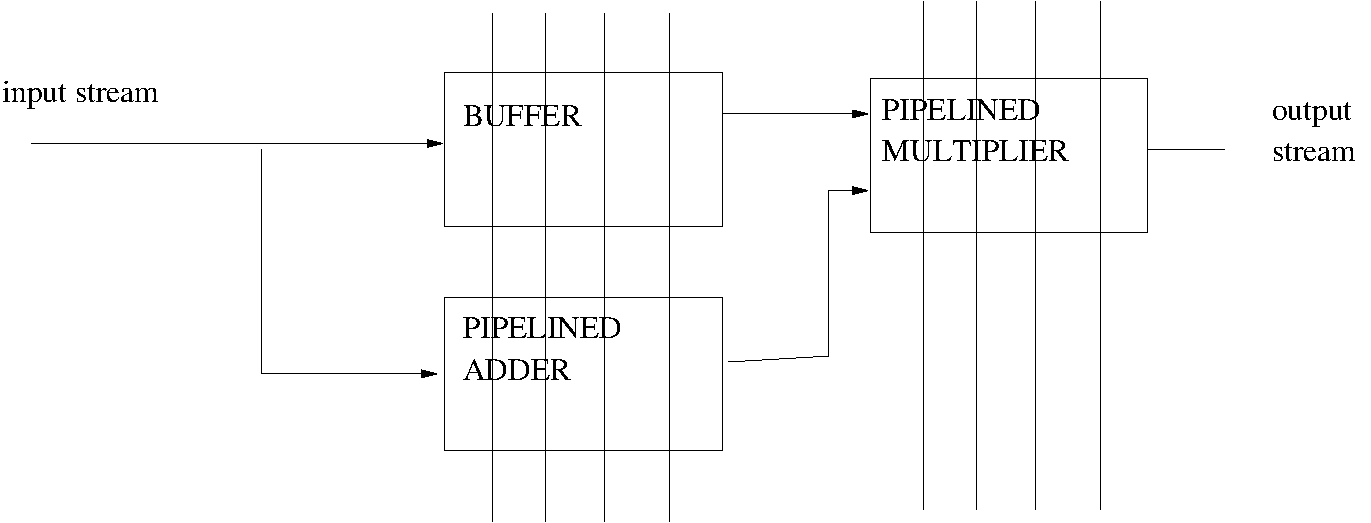
\includegraphics[width=9cm]{figs/ExpectedHardware.pdf}
  \caption{The hardware we would like to see.}
\end{figure}

}

\frame[containsverbatim]{\frametitle{The AHIR  tools produce the expected hardware}
\begin{verbatim}
void __loop_pipelining_on__(int,int,int);
void Daemon()
{
  while(1)
  {
    // tell the AHIR compiler to pipeline this loop..
    // and keep 32 iterations alive at any time.
    __loop_pipelining_on__(32,2,1);

    float a = read_float32("a_pipe");
    float ap1 = (a + 1.0);
    float result = a*ap1;
    write_float32("result_pipe", result);
  }
}
\end{verbatim}

}


\frame[containsverbatim]{\frametitle{Loop Pipelining}
\begin{itemize}
\item The  AHIR compiler modifies the control path to
allow multiple iterations of the loop to be active simultaneously.
\item While doing this, all dependencies must be taken care of.
\begin{itemize}
\item Operation order.
\item Data dependency.
\item Memory accesses.
\item Pipe accesses.
\item Producer-consumer dependencies are the key.
\end{itemize}
\item The data-path is modified by inserting buffers to balance
the pipeline.
\end{itemize}
}

\frame[containsverbatim]{\frametitle{Control path modifications}
\begin{figure}
  \centering
  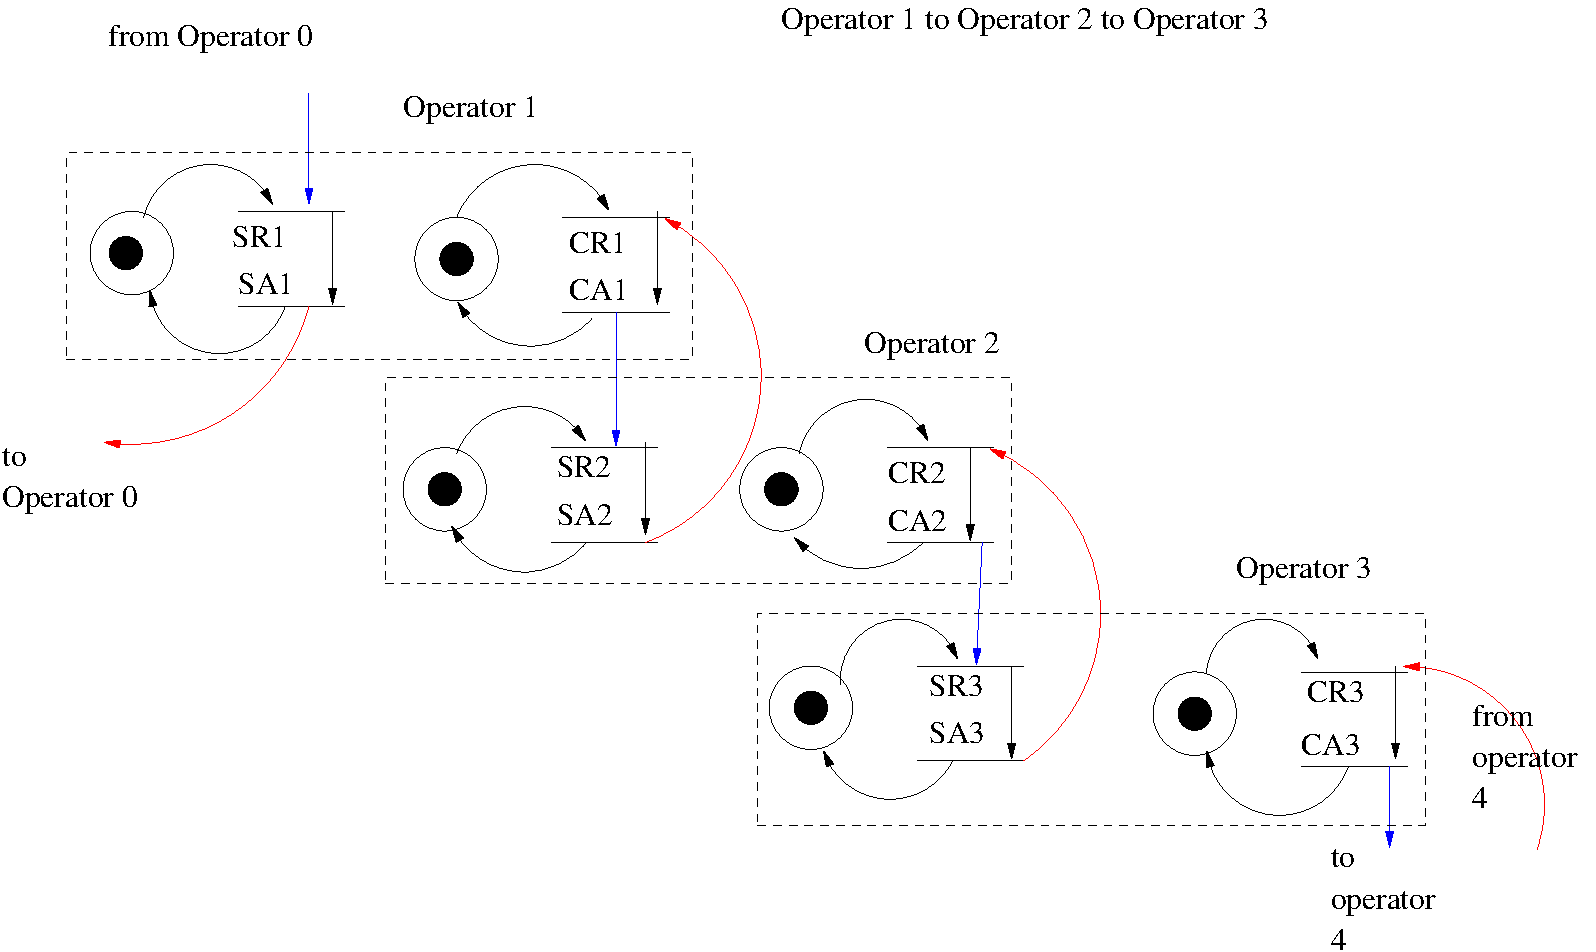
\includegraphics[width=9cm]{figs/ProducerConsumer.pdf}
  \caption{Producer consumer dependencies in the pipeline}
\end{figure}
}

\frame[containsverbatim]{\frametitle{Cost of loop pipelining}
\begin{itemize}
\item In the data-path: additional buffering.
\item In the control-path, the cost of each join increases by
a factor of $\log N$, where $N$ is the number of iterations that
need to be kept alive.
\item Need to choose $N$ carefully and avoid unbalanced loop bodies
in order to manage cost of loop pipelining.
\item Performance benefits can be substantial.
\end{itemize}
}

\frame[containsverbatim]{\frametitle{An example with and without loop-pipelining}

\begin{itemize}
\item Look at ex1/ and ex1\_no\_loop\_pipeling to see the difference.
\item More than 20X speedup by pipelining the loop.
\end{itemize}
}

\frame[containsverbatim]{\frametitle{Loop-pipelining is critical!}
\begin{itemize}
\item  Think of the hardware as interacting threads, each of which
is a pipelined loop.
\end{itemize}
}


\end{document}
